\section{Appendix Organization}

The appendix follows the same experimental progression as the main paper. We
begin with RFNN spectra, which isolate the kernel-level four-bulk mechanism
under controlled synthetic data. We then turn to trainable synthetic MLPs,
where the same latent-buffer idea is measured through memorization fraction and
score error over optimization. Finally, we give the VAE and latent-diffusion
diagnostics for CelebA and CIFAR-10, including reconstruction checks, FID,
per-dimension memorization trajectories, a spatial-DiT pilot, and the
frozen-latent spectrum memorization predictor.

\section{Experimental Details}
\label{app:protocol}
\label{app:methods}

\paragraph{Synthetic latent data.}
The synthetic experiments draw a low-dimensional signal subspace with
dimension $\dint$ and embed it in an observed latent space of dimension
$\dlat$. Unless noted otherwise, the signal coordinates are sampled from an
anisotropic Gaussian mixture and the remaining coordinates receive independent
null noise. The nonlinear random-feature experiments use the same data design
but study the spectrum of the feature kernel rather than generated samples.
The trainable synthetic MLP experiments use the analytic Gaussian score as the
target, which is why we report score error rather than image FID.

\paragraph{Synthetic experiment details.}
For Experiment~1, we fix $\dint=5$ and sweep $\dlat$, so the exact null-buffer
size is $\dlat-\dint$. For Experiment~2, we fix the observed latent space at
$\dlat=20$ and sweep $\dint$, so the exact null-buffer size decreases until it
vanishes at $\dint=\dlat$. The default RFNN data are anisotropic GMM samples
with $\sigma_{\rm signal}=1.0$, $\sigma_\perp=0.5$, center scale $3.0$,
$n=500$, diffusion time $t=0.01$, and $K$ Monte Carlo diffusion-noise samples used to estimate $\Umat$ ($K=50$ for the $\pwidth=64\dlat$ raw-data spectra, $K=500$ for the $\pwidth=\dlat+\nsamp+300$ set; see each run's \texttt{config.json}). The $K$-draw average has full rank $\pwidth$ with a soft shoulder at index $\nsamp$; the single-draw matrix has exactly $\pwidth-\nsamp$ zero eigenvalues. The Gaussian robustness panels remove mixture centers
and either sweep $\sigma_\perp\in\{0.1,0.3,0.5\}$ at fixed
$\sigma_{\rm signal}=1.0$, or sweep
$\sigma_{\rm signal}\in\{0.5,1.0,1.5\}$ at fixed $\sigma_\perp=0.3$.
The synthetic MLP uses the same $\dint=5$, $n=500$, $\sigma_\perp=0.5$
latent-distribution family as the main RFNN sweep, trains a fixed-hidden-width
score MLP for 5M steps over seeds 42--46, and evaluates sample recall by the
nearest-neighbor ratio on generated synthetic samples.

\paragraph{Width controls.}
\label{app:width-controls}
The RFNN spectra are reported under three width rules:
$p=64\dlat$, $p=\dlat+n+300$, and fixed $p=1800$ with fixed total null energy.
The first setting checks a high-feature-count regime. The second grows width just enough to cover the $\nsamp$ data-supported directions plus a $\dlat+300$ margin, so $\psi_p=\pwidth/\dlat$ approaches $1$ at large $\dlat$ and the noise-dimension block broadens accordingly. The
fixed-width/fixed-energy control removes the two main confounds in the $\dlat$
sweep: increasing model width and increasing total injected null variance.

\paragraph{Memorization metric.}
A generated sample $\hat x$ is counted as memorized when the ratio of its distances to its nearest and second-nearest training points, $\|\hat x-\mathrm{NN}_1\|/\|\hat x-\mathrm{NN}_2\|$, is below $1/3$, the nearest-neighbor ratio criterion of \citet{bonnaire2025} (see also \citealp{somepalli2023diffusion}). Synthetic experiments apply it in latent space; image experiments apply it in pixel space to decoded samples. The relevant comparison set is the training subset used
by the diffusion model, not the full VAE training set. Reported curves are the
mean across five seeds with confidence bands unless the caption states that the
figure is a deterministic VAE diagnostic.

\paragraph{VAE reconstruction memorization as an intrinsic-dimension proxy.}
Before training diffusion, we pass the same diverse 1k subset through each
frozen VAE and apply the pixel-space nearest-neighbor ratio to the immediate
reconstructions. This is not diffusion memorization. It measures whether the
VAE bottleneck preserves enough sample identity for any downstream pixel-space
memorization test to be meaningful. We use the rise and plateau of this
reconstruction-memorization curve as a practical proxy for the dataset's
effective intrinsic-dimensionality threshold: below that point the latent code
is capacity-limited, while above it increasing $\dlat$ mostly adds excess
buffer dimensions.

\paragraph{Real-data VAEs.}
CelebA and CIFAR-10 experiments first train one VAE per latent dimension on the
full available training split, not on the 1k diffusion subset. The VAE is a
five-stage convolutional encoder/decoder with channel widths
$(32,64,128,256,512)$. The final checkpoints use the ResNet-style variant:
stride-two convolutional downsampling, GroupNorm/SiLU residual blocks,
transpose-convolution upsampling, and a Tanh output. CelebA uses 21k training
and 6k validation images from the local CelebA-HQ tar split at $32\times32$
grayscale resolution; CIFAR-10 uses the standard 50k/10k train/test split at
$32\times32$ RGB resolution. The objective combines reconstruction with a KL
penalty to the standard normal prior. In the capacity-loss form used by the
final checkpoints, $\mathcal L_{\rm VAE}=\mathcal L_{\rm recon}+
\gamma|\mathrm{KL}-C(t)|$, with $C(t)$ warmed up early in training; the logs
also record $\beta$, reconstruction MSE/L1, KL, learning-rate reductions, and
early stopping. This is why the appendix reports VAE reconstruction
memorization before any diffusion result: if encode/decode alone cannot
preserve sample identity, a pixel-space memorization test on generated samples
is not yet meaningful.

\paragraph{Real-data latent diffusion.}
After selecting the best VAE checkpoint by validation objective, we encode the
same farthest-first diverse 1k subset for each dataset and train a latent-space
MLP score model on those codes. The final reported runs use a depth-five MLP with hidden width 1024, sinusoidal time features, SGD with learning rate
$10^{-3}$ and momentum $0.80$, batch size 512, and a 5M-step horizon over five
seeds. The hidden width is fixed across $\dlat$, so increasing the latent
dimension changes the input/output dimension and the amount of latent buffer,
but not the dominant hidden-layer capacity. Training loss is logged every 10k
steps; memorization and FID are evaluated every 100k steps using 10k generated samples, with the same 1k training subset as the FID reference.

\paragraph{Spatial-DiT pilot.}
The appendix also includes a CelebA pilot that replaces the vector VAE/MLP
pipeline with a spatial $4\times4$ VAE and an unconditional DiT-style score
model. In that setting the plotted $\dlat$ is a channel count, so a single
step in $\dlat$ changes the latent state by $16$ scalar coordinates. This
makes the sweep harder to tune and interpret than the vector-latent MLP
experiments: changing the channel count changes the scalar latent dimension,
the VAE decoder, the first and last DiT projections, and the second-order
cross-position/cross-channel covariance structure that the transformer sees.
The DiT pilot therefore tests whether the buffer idea leaves a trace in a
more realistic image architecture, not whether the clean vector-latent theory
transfers without modification.

\paragraph{Optimization failures and clipped diagnostics.}
Nonfinite runs are treated as failed optimization runs, not as evidence of zero
memorization. Gradient clipping was useful diagnostically because it prevented
some high-dimensional CIFAR-10 runs from producing NaNs, but it also suppressed
memorization almost entirely. The clean CIFAR-10 aggregate therefore uses
unclipped replacement seeds with the same SGD hyperparameters rather than
mixing clipped and unclipped regimes.

\FloatBarrier

\section{RFNN Spectral Diagnostics}
\label{app:rfnn-clean}
\label{app:appendix-figures}

The RFNN experiments are spectral diagnostics, not sampled diffusion runs. They
therefore do not have an image-level memorization percentage. Their purpose is
to check whether the kernel spectrum separates into the predicted signal,
latent-null, sample, and rank-null regions under the same data choices used by
the trainable experiments.

Experiment~2, the source-dimensionality sweep, uses the updated synthetic
parameters from the final rerun: $\dlat$ is fixed at 20, $\dint$ ranges over
$\{2,5,8,12,16,20,25,30,35,40\}$, and the whole sweep is repeated under
$p=64\dlat$, $p=\dlat+n+300$, and fixed-$p$ width controls. This experiment is
the reverse of Experiment~1, the main $\dlat$ sweep. It asks whether the noise-dimension block
shrinks when more of the fixed observed latent space is occupied by true source
variation, and whether over-intrinsic source structure merely compresses into
the fixed observed space rather than creating additional observed signal modes.

\newcommand{\rfnnBulkColorKey}{Colors are assigned by sorted eigenvalue-index
blocks rather than fitted clusters: red denotes signal/source modes, green the
observed latent-null/noise-dimension block, blue sample-specific modes, and
purple rank-null modes. Dashed vertical lines mark the median log-eigenvalue of
each colored block.}

\begin{figure}[!htbp]
  \centering
  
\includegraphics[width=0.96\linewidth]{figures/rfnn_exp2_p64.pdf}
  \caption{Experiment~1 RFNN four-bulk spectra for the latent-dimension sweep with
  $p=64\dlat$. Here $\dint=5$, $\sigma_{\rm signal}=1.0$,
  $\sigma_\perp=0.5$, GMM center scale is $3.0$, and the swept variable is
  $\dlat\in\{5,10,20,40,100,200,500,1000\}$. Each panel plots the eigenvalue histogram after assigning
  eigenmodes to the signal, latent-null, sample, and rank-null index regions
  predicted by the theory. This highly overcomplete feature setting checks that
  the expected spectral ordering is visible when the RFNN has many more
  features as $\dlat$ grows. Since the synthetic $\dint=5$ is known exactly,
  the green block grows in the exact increasing-buffer regime
  $\dlat-\dint$, with little irregular variation beyond the deterministic
  change in block size. \rfnnBulkColorKey}
  \label{fig:app-rfnn-exp2-widths}
\end{figure}

\begin{figure}[!htbp]
  \centering
  
\includegraphics[width=0.96\linewidth]{figures/rfnn_exp2_pndr.pdf}
  \caption{Experiment~1 RFNN four-bulk spectra for the latent-dimension sweep with
  $p=\dlat+n+300$. The data sweep is the same as
  Figure~\ref{fig:app-rfnn-exp2-widths}: fixed $\dint=5$, fixed
  $\sigma_\perp=0.5$, and increasing $\dlat$. This width grows just enough to represent the latent,
  sample, and rank-null regions, so it checks that the four-bulk ordering does
  not require the much wider $p=64\dlat$ feature map. The persistence of the
  same qualitative separation supports the interpretation that the effect comes
  from the latent-buffer geometry rather than from overcomplete RFNN width.
  The same near-monotone growth of the green block with the exact buffer size
  $\dlat-\dint$ appears even in this controlled-width setting. \rfnnBulkColorKey}
  \label{fig:app-rfnn-exp2-pndr}
\end{figure}

\begin{figure}[!htbp]
  \centering
  
\includegraphics[width=0.96\linewidth]{figures/rfnn_exp2_pfixed.pdf}
  \caption{Experiment~1 RFNN four-bulk spectra for the latent-dimension sweep with fixed
  $p=1800$ and fixed total null energy. The swept variable is still $\dlat$,
  but $\sigma_\perp^2$ is rescaled as
  $E_{\rm null}/(\dlat-\dint)$ so that the total null variance does not grow
  with latent dimension. This is the strictest control because
  increasing $\dlat$ no longer increases either the number of random features or
  the total variance injected into null coordinates. The remaining spectral
  separation is therefore the cleanest evidence that the buffer arises from the
  distribution of modes across the latent space. The increasing regime is tied
  to the exact synthetic quantity $\dlat-\dint$, not to increasing RFNN width or
  total null energy. \rfnnBulkColorKey}
  \label{fig:app-rfnn-exp2-pfixed}
\end{figure}

\begin{figure}[!htbp]
  \centering
  
\includegraphics[width=0.96\linewidth]{figures/rfnn_exp3_over_p64.pdf}
  \caption{Experiment~2 RFNN source-dimensionality sweep with a fixed observed latent space
  under the $p=64\dlat$ width rule. The learned latent dimension is held fixed
  at $\dlat=20$, $\sigma_{\rm signal}=1.0$, $\sigma_\perp=0.5$, and GMM
  center scale $3.0$, while the intrinsic dimension of the source distribution
  sweeps $\dint\in\{2,5,8,12,16,20,25,30,35,40\}$. When
  $\dint<\dlat$, the remaining observed coordinates form a genuine null buffer;
  as $\dint$ approaches $\dlat$, that buffer shrinks and the signal and sample
  regions become less separated. Because $\dlat=20$ is fixed and known, this is
  the exact decreasing-buffer regime: the green block shrinks as
  $\dlat-\dint$ and disappears at $\dint=\dlat$. \rfnnBulkColorKey}
  \label{fig:app-rfnn-exp3-widths}
\end{figure}

\begin{figure}[!htbp]
  \centering
  
\includegraphics[width=0.96\linewidth]{figures/rfnn_exp3_over_pndr.pdf}
  \caption{Experiment~2 RFNN source-dimensionality sweep with $p=\dlat+n+300$. This panel uses
  the same fixed observed latent space as Figure~\ref{fig:app-rfnn-exp3-widths}
  and the same $\dint$ sweep, but removes the highly overcomplete
  feature-count scaling. The same loss of
  separation as $\dint$ approaches $\dlat$ shows that the effect is not specific
  to the widest RFNN parameterization. The smooth decrease of the null-buffer
  block with the exact gap $\dlat-\dint$ is the key diagnostic. \rfnnBulkColorKey}
  \label{fig:app-rfnn-exp3-pndr}
\end{figure}

\begin{figure}[p]
  \centering
  
\includegraphics[width=0.96\linewidth]{figures/rfnn_exp3_over_pfixed.pdf}
  \caption{Experiment~2 RFNN source-dimensionality sweep with fixed width. For
  this control $\dlat=20$ is fixed and $\dint$ is swept as in the other
  Experiment~2 panels, while RFNN width is held fixed instead of growing with
  $\dlat$ or $\dint$. For $\dint>\dlat$, the source structure is compressed into the fixed observed
  latent space, so the high-$\dint$ regime should be read as an over-intrinsic
  stress test rather than a literal null-buffer regime. The fixed-width control
  makes the narrowing of the buffer visible without simultaneously changing
  RFNN capacity. The relevant regime is therefore decreasing until the exact
  boundary $\dint=\dlat$, followed by compressed over-intrinsic behavior rather
  than a new buffer. \rfnnBulkColorKey}
  \label{fig:app-rfnn-exp3-pfixed}
\end{figure}

\begin{figure}[p]
  \centering
  
\includegraphics[width=0.96\linewidth]{figures/rfnn_exp2_robust_sigma_pndr.pdf}
  \caption{Experiment~1 RFNN latent-dimension sweep on pure anisotropic Gaussian data while
  varying the null-noise scale. Rows use
  $\sigma_\perp\in\{0.1,0.3,0.5\}$ at fixed $\dint=5$,
  $\sigma_{\rm signal}=1.0$, and swept $\dlat$. This test removes mixture structure from the
  synthetic data and checks that the four-bulk decomposition is not an artifact
  of the default GMM. Increasing null noise shifts the latent-null region and
  changes the gap to the sample region, as expected from the buffer
  interpretation. \rfnnBulkColorKey}
  \label{fig:app-rfnn-robustness}
\end{figure}

\begin{figure}[p]
  \centering
  
\includegraphics[width=0.96\linewidth]{figures/rfnn_exp2_robust_sigscale_pndr.pdf}
  \caption{Experiment~1 RFNN latent-dimension sweep on pure anisotropic Gaussian data while
  varying the signal scale. Rows use
  $\sigma_{\rm signal}\in\{0.5,1.0,1.5\}$ at fixed $\dint=5$,
  $\sigma_\perp=0.3$, and swept $\dlat$. The signal block moves with the strength of the
  structured coordinates, while the sample and null regions remain governed by
  the latent buffer and noise statistics. This confirms that the visible bulk
  ordering responds to the intended data-level parameters. \rfnnBulkColorKey}
  \label{fig:app-rfnn-robust-sigscale}
\end{figure}

\begin{figure}[p]
  \centering
  
\includegraphics[width=0.96\linewidth]{figures/rfnn_exp3_robust_sigma_pndr.pdf}
  \caption{Experiment~2 RFNN source-dimensionality sweep on pure anisotropic Gaussian data
  while varying the null-noise scale. Rows use
  $\sigma_\perp\in\{0.1,0.3,0.5\}$ at fixed $\dlat=20$ and
  swept $\dint$. The same buffer-collapse pattern appears
  when $\dint$ approaches the fixed observed latent dimension, and the amount of
  separation between null and sample regions changes with the null-noise scale.
  \rfnnBulkColorKey}
  \label{fig:app-rfnn-robust-dint-sigma}
\end{figure}

\begin{figure}[p]
  \centering
  
\includegraphics[width=0.96\linewidth]{figures/rfnn_exp3_robust_sigscale_pndr.pdf}
  \caption{Experiment~2 RFNN source-dimensionality sweep on pure anisotropic Gaussian data
  while varying the signal scale. Rows use
  $\sigma_{\rm signal}\in\{0.5,1.0,1.5\}$ at fixed $\dlat=20$,
  $\sigma_\perp=0.3$, and swept $\dint$. Larger signal scale sharpens the leading
  signal region, but the qualitative transition as $\dint$ approaches $\dlat$
  remains governed by the amount of available null-buffer dimension.
  \rfnnBulkColorKey}
  \label{fig:app-rfnn-robust-dint-sigscale}
\end{figure}

\paragraph{Feature-scale caveat for RFNN spectra.}
The nonlinear feature map is kept as $\tanh$, but the data scale is chosen to
avoid saturation. If the preactivations saturate, the predicted four-bulk
structure can fragment into extra internal sub-bulks. These saturation-induced
sub-bulks reflect the feature nonlinearity being driven outside its
approximately linear regime, not an additional latent-buffer effect.

\FloatBarrier

\section{Synthetic MLP Diagnostics}
\label{app:synthetic-mlp-clean}

The synthetic MLP figures use five seeds, a 5M-step training horizon, and the
nearest-neighbor memorization ratio described in Appendix~\ref{app:protocol}.
This appendix repeats the main fixed-width sweep with the larger latent range
$\dlat\in\{5,8,10,12,15,20,25,30,35,40,60,80,100,120,140,160,180,200,220,240\}$.
We report memorization percentage over training steps so that the onset,
growth, and saturation of memorization remain visible.

\begin{figure}[!htbp]
  \centering
  
\includegraphics[width=0.92\linewidth]{figures/synthetic_mlp_mem_over_steps_full.pdf}
  \caption{Synthetic trainable MLP memorization trajectories across latent
  dimension. The curves show when each model begins to reproduce
  individual training samples according to the nearest-neighbor ratio, while
  retaining the full shape of the rise rather than collapsing it to a single
  threshold. Smaller latent dimensions memorize quickly because the model
  reaches sample-specific directions after absorbing only a short null buffer;
  larger latent dimensions delay this rise, consistent with the RFNN picture
  that additional null directions must be learned before sample-specific modes
  dominate. The extended sweep shows that this continues through
  $\dlat=240$ under the fixed-width MLP control. The sweep is almost ordered by the exact synthetic buffer size
  $\dlat-\dint$: after the no-buffer $\dlat=\dint=5$ case, increasing $\dlat$
  produces a steadily lower and later memorization regime rather than large
  dimension-to-dimension variation.}
  \label{fig:app-synthetic-mlp-mem}
\end{figure}

\begin{figure}[!htbp]
  \centering
  \begin{subfigure}{0.48\linewidth}
    
\includegraphics[width=\linewidth]{figures/synthetic_mlp_final_mem_ratio_full.pdf}
    \caption{Final memorization at 5M steps.}
  \end{subfigure}
  \begin{subfigure}{0.48\linewidth}
    
\includegraphics[width=\linewidth]{figures/synthetic_mlp_max_mem_ratio_full.pdf}
    \caption{Peak memorization during training.}
  \end{subfigure}
  
\includegraphics[width=0.70\linewidth]{figures/synthetic_mlp_max_mem_hist_full.pdf}
  \caption{Synthetic MLP final and peak memorization summaries. The final
  memorization fraction measures the end-of-training state, while the peak
  memorization fraction captures transient sample recall that may not persist
  until 5M steps. The seed-level histogram exposes how much of the latent
  dimensional trend is stable across random seeds rather than being driven by a
  single unusually memorizing run. The final and peak summaries both support
  the same decreasing regime with increasing $\dlat$, including the high-dimensional extension beyond the
  main-text $\dlat\le 40$ view.}
  \label{fig:app-synthetic-mlp-mem-summary}
\end{figure}

\begin{figure}[!htbp]
  \centering
  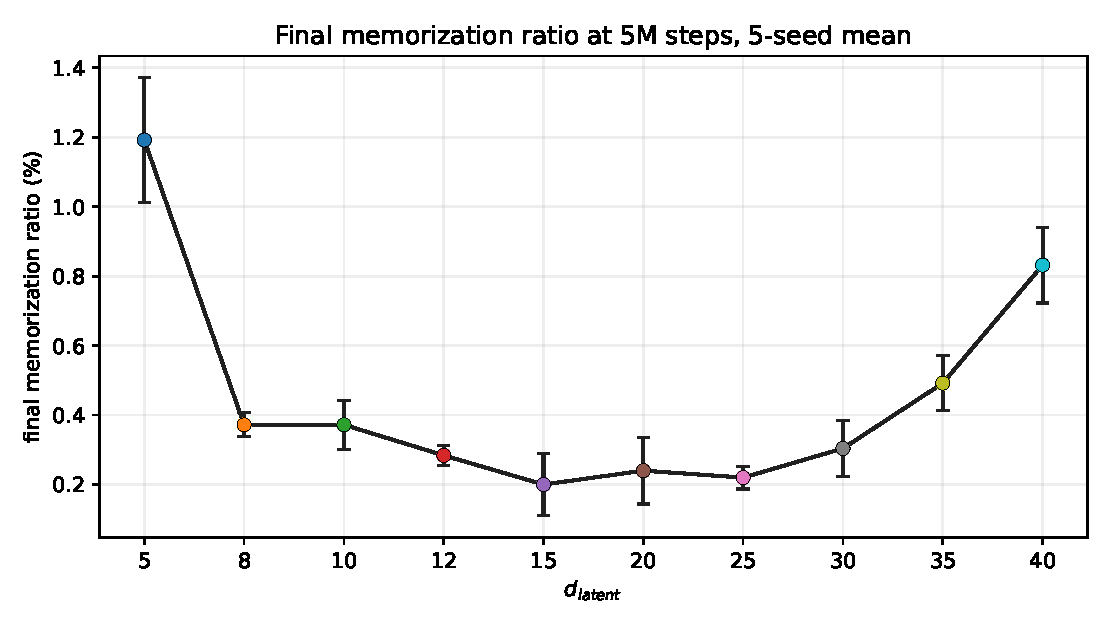
\includegraphics[width=0.62\linewidth]{figures/synthetic_mlp_final_mem_ratio_scaled8d.pdf}
  \caption{Width-scaled control for \cref{fig:synthetic-mlp-main}: the same sweep with hidden width $8\dlat$ (40 to 320) instead of a fixed $256$, five seeds, 5M steps. Memorization sits at the $1\%$ level and rises again for $\dlat\ge30$ as the network grows, so a width-scaled sweep is a capacity sweep and does not isolate the latent dimension. This is why the main text holds the width fixed.}
  \label{fig:app-synthetic-mlp-scaled}
\end{figure}

\begin{figure}[!htbp]
  \centering
  \begin{subfigure}{0.48\linewidth}
    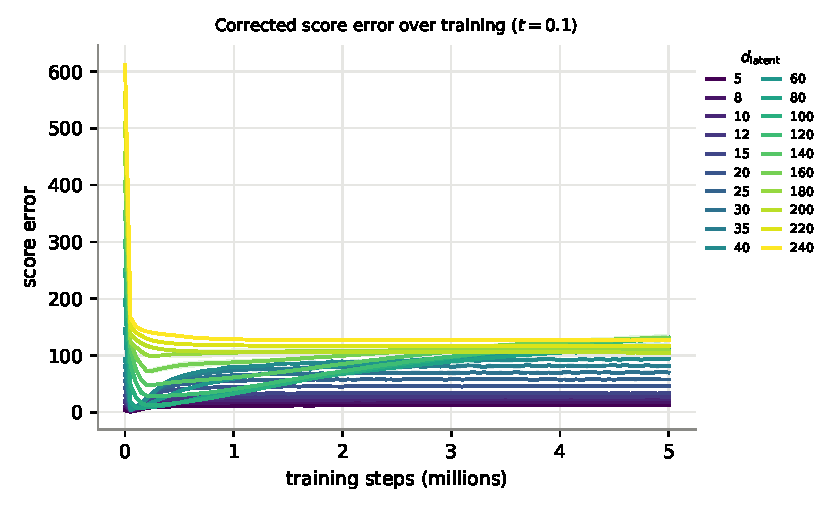
\includegraphics[width=\linewidth]{figures/synthetic_mlp_score_error_full.pdf}
    \caption{Score error, all coordinates.}
  \end{subfigure}
  \begin{subfigure}{0.48\linewidth}
    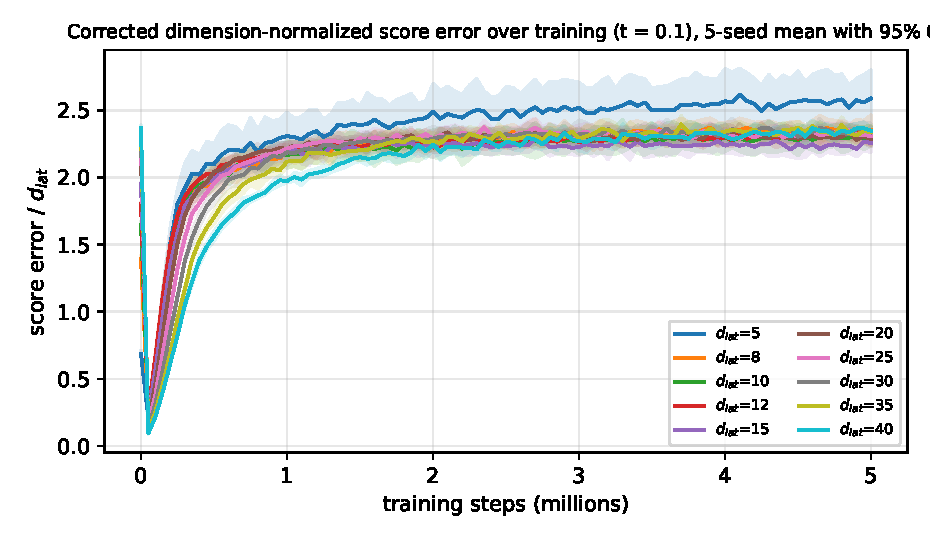
\includegraphics[width=\linewidth]{figures/synthetic_mlp_score_error_per_dim_full.pdf}
    \caption{Score error normalized per latent dimension.}
  \end{subfigure}
  \caption{Synthetic MLP score-error diagnostics: the population score error at $t=0.1$ against the exact GMM score on a held-out set, five-seed mean with 95\% CI, over the complete fixed-width sweep $\dlat=5$--$240$ (the main-text panel of \cref{fig:synthetic-mlp-main} covers $\dlat\le 40$). The left panel sums over all latent coordinates; the right panel divides by $\dlat$, which removes the mechanical scaling with $\dlat$.
  This distinction matters because a larger latent space has more coordinates
  to predict even if the average coordinate-wise error is comparable. Score
  error is the appropriate quality metric in this synthetic setting because the
  target distribution is specified analytically in latent space rather than
  through decoded images. Beyond $\dlat\approx 60$ the per-coordinate error has
  not returned to its small-$\dlat$ plateau by the 5M-step horizon: it ends at
  $2.59$ for $\dlat=5$ but $0.53$ for $\dlat=240$, so the widest latents never
  begin the divergence from the population score that accompanies memorization
  at small $\dlat$.}
  \label{fig:app-synthetic-mlp-score}
\end{figure}

\paragraph{Interpreting threshold-free memorization curves.}
Single hitting times such as $\tau_{\rm mem}$ are convenient summaries, but
they hide whether a run crosses a threshold sharply, gradually, or only
transiently. The full memorization-fraction curves are therefore the primary
diagnostic for the trainable MLP experiments. Thresholded hitting times are
used later only in the spectral-predictor analysis, where multiple fixed
memorization levels are compared against predicted iso-memorization times.

\FloatBarrier

\section{Real-Data VAE Diagnostics}
\label{app:vae-clean}

The real-data experiments separate two questions. First, the VAE must preserve
enough image identity that nearest-neighbor memorization can be detected after
encoding and decoding. Second, the diffusion model must have enough capacity
and stable optimization to actually memorize the encoded subset. For this
reason, the VAE figures appear before the diffusion figures: they determine
which latent dimensions are still below the effective intrinsic dimensionality
of the image manifold and therefore should not be expected to obey the
excess-buffer prediction cleanly.

\begin{figure}[!htbp]
  \centering
  \begin{subfigure}{0.48\linewidth}
    
\includegraphics[width=\linewidth]{figures/vae_diagnostics/celeba_reconstruction_mem_vs_d.pdf}
    \caption{CelebA reconstruction memorization.}
  \end{subfigure}
  \begin{subfigure}{0.48\linewidth}
    
\includegraphics[width=\linewidth]{figures/vae_diagnostics/cifar10_reconstruction_mem_vs_d.pdf}
    \caption{CIFAR-10 reconstruction memorization.}
  \end{subfigure}
  \begin{subfigure}{0.48\linewidth}
    
\includegraphics[width=\linewidth]{figures/vae_diagnostics/celeba_vae_metrics_vs_d.pdf}
    \caption{CelebA VAE loss terms.}
  \end{subfigure}
  \begin{subfigure}{0.48\linewidth}
    
\includegraphics[width=\linewidth]{figures/vae_diagnostics/cifar10_vae_metrics_vs_d.pdf}
    \caption{CIFAR-10 VAE loss terms.}
  \end{subfigure}
  \caption{VAE diagnostics across latent dimension for CelebA and CIFAR-10.
  The reconstruction-memorization panels encode the 1k diffusion subset through
  the frozen VAE and decode it immediately, then apply the same pixel-space KNN
  ratio used for generated samples. This measures whether the VAE bottleneck
  itself preserves enough sample identity for memorization to be detectable.
  The loss panels show the corresponding validation reconstruction and KL
  behavior across dimensions for VAEs trained on the full training split.
  Low-dimensional VAEs blur or average away identity, so weak diffusion
  memorization at small $\dlat$ can reflect a lossy representation rather than
  an intrinsically nonmemorizing diffusion model. In real data the intrinsic
  dimension is only approximate, but the reconstruction panels show the first
  regime cleanly: identity preservation increases with $\dlat$ until the VAE is
  near the effective intrinsic dimensionality. Below that point, the model is
  capacity-limited and the spectral memorization predictor is not expected to
  follow the empirical curve closely.}
  \label{fig:app-vae-metrics}
\end{figure}

\begin{figure}[p]
  \centering
  
\includegraphics[width=0.96\linewidth,height=0.69\textheight,keepaspectratio]{figures/vae_diagnostics/celeba_vae_reconstruction_contact_sheet.pdf}
  \caption{CelebA VAE encode/decode contact sheet. The rows show original
  images and their final checkpoint reconstructions across latent dimensions,
  making visible the point at which identity-level facial features become
  stable under the VAE bottleneck. The visual trend is mostly increasing rather
  than noisy: larger $\dlat$ steadily moves the VAE toward the approximate
  intrinsic-image regime where sample identity survives encode/decode. This
  qualitative check is necessary because
  the downstream KNN memorization metric can only detect sample recall when
  reconstructions preserve enough pixel-level identity.}
  \label{fig:app-vae-celeba-contact}
\end{figure}

\begin{figure}[p]
  \centering
  
\includegraphics[width=0.96\linewidth,height=0.69\textheight,keepaspectratio]{figures/vae_diagnostics/cifar10_vae_reconstruction_contact_sheet.pdf}
  \caption{CIFAR-10 VAE encode/decode contact sheet. The rows show original
  images and final checkpoint reconstructions. CIFAR-10 has much more class and
  texture variation than the CelebA subset, so visual reconstruction quality is
  an important check before interpreting downstream diffusion memorization. The
  higher-dimensional VAEs preserve more object identity and local structure,
  making pixel-space nearest-neighbor tests more meaningful. As with CelebA,
  reconstruction quality is best read as an increasing-capacity regime up to an
  approximate effective intrinsic dimension, not as arbitrary variation across
  latent widths.}
  \label{fig:app-vae-cifar-contact}
\end{figure}

\begin{figure}[!htbp]
  \centering
  \begin{subfigure}{0.48\linewidth}
    
\includegraphics[width=\linewidth]{figures/vae_diagnostics/celeba_vae_training_curves.pdf}
    \caption{CelebA VAE training curves.}
  \end{subfigure}
  \begin{subfigure}{0.48\linewidth}
    
\includegraphics[width=\linewidth]{figures/vae_diagnostics/cifar10_vae_training_curves.pdf}
    \caption{CIFAR-10 VAE training curves.}
  \end{subfigure}
  \caption{VAE training curves for CelebA and CIFAR-10. The reported VAE
  checkpoints are selected by validation objective after the reconstruction and
  KL objectives have largely stabilized, so the downstream latent-diffusion
  trends are not simply caused by comparing undertrained encoders at different
  latent dimensions. Together with
  Figures~\ref{fig:app-vae-metrics}--\ref{fig:app-vae-cifar-contact}, these
  diagnostics justify treating high-dimensional VAE latents as a meaningful
  substrate for pixel-space memorization tests.}
  \label{fig:app-vae-quality}
\end{figure}

\FloatBarrier

\section{Real-Data Diffusion Diagnostics}
\label{app:real-diffusion-clean}

\begin{figure}[!htbp]
  \centering
  \begin{subfigure}{0.48\linewidth}
    
\includegraphics[width=\linewidth]{figures/celeba_loss_over_steps_ci.pdf}
    \caption{CelebA diffusion loss.}
  \end{subfigure}
  \begin{subfigure}{0.48\linewidth}
    
\includegraphics[width=\linewidth]{figures/cifar10_loss_over_steps_ci.pdf}
    \caption{CIFAR-10 diffusion loss.}
  \end{subfigure}
  \begin{subfigure}{0.48\linewidth}
    
\includegraphics[width=\linewidth]{figures/cifar10_final_loss_vs_d.pdf}
    \caption{CIFAR-10 final loss by $\dlat$.}
  \end{subfigure}
  \begin{subfigure}{0.48\linewidth}
    
\includegraphics[width=\linewidth]{figures/cifar10_score_loss_per_dim_over_steps_ci.pdf}
    \caption{CIFAR-10 score loss per dimension.}
  \end{subfigure}
  \caption{Optimization diagnostics for the real-data diffusion runs, shown
  before the memorization and FID panels because they establish that the models
  are actually training. The loss curves track whether differences in
  memorization and FID coincide with gross optimization failure, while the
  CIFAR-10 per-dimension score loss removes the trivial scaling of the
  objective with latent dimension. Gradient clipping was used only as a
  diagnostic intervention: it prevented some unstable runs from diverging, but
  it also strongly suppressed memorization and therefore changed the effective
  training regime. The aggregate CIFAR-10 results are reported using stable
  unclipped runs so that optimizer changes are not conflated with
  latent-dimensional effects.}
  \label{fig:app-real-optimization}
\end{figure}

\begin{figure}[!htbp]
  \centering
  \begin{subfigure}{0.48\linewidth}
    
\includegraphics[width=\linewidth]{figures/celeba_mem_over_steps_ci.pdf}
    \caption{CelebA memorization.}
  \end{subfigure}
  \begin{subfigure}{0.48\linewidth}
    
\includegraphics[width=\linewidth]{figures/cifar10_mem_over_steps_ci.pdf}
    \caption{CIFAR-10 memorization.}
  \end{subfigure}
  \begin{subfigure}{0.48\linewidth}
    
\includegraphics[width=\linewidth]{figures/celeba_fid_over_steps_ci.pdf}
    \caption{CelebA FID.}
  \end{subfigure}
  \begin{subfigure}{0.48\linewidth}
    
\includegraphics[width=\linewidth]{figures/cifar10_fid_over_steps_ci.pdf}
    \caption{CIFAR-10 FID.}
  \end{subfigure}
  \caption{Real-data diffusion trajectories with five-seed confidence bands.
  The memorization panels report the fraction of generated samples that pass the
  pixel-space nearest-neighbor ratio against the diffusion training subset. The
  FID panels report image-quality evolution over the same optimization horizon.
  Reading the two rows together separates quality improvement from direct
  sample recall: a model can improve FID before it begins to reproduce exact
  training examples, and a high-dimensional latent can delay memorization even
  when the generated samples are already becoming visually plausible. Across
  $\dlat$, memorization follows a clean increasing-then-decreasing regime near
  the approximate effective intrinsic dimension, while FID follows the
  complementary decreasing-then-increasing regime: quality improves as the VAE
  bottleneck is relieved and worsens again when the latent score problem is too
  wide.}
  \label{fig:app-real-trajectories}
\end{figure}

\begin{figure}[p]
  \centering
  
\includegraphics[width=0.94\linewidth,height=0.72\textheight,keepaspectratio]{figures/celeba_individual_mem_by_d_over_steps.pdf}
  \caption{CelebA per-dimension memorization trajectories. Each panel
  isolates one latent dimension and shows the seed-level evolution of KNN
  memorization over the 5M-step run. This view is important because the
  aggregate curve can hide whether a dimension memorizes consistently across
  seeds or only through a few high-memorization runs. At very small $\dlat$, the
  simple latent-buffer prediction need not apply cleanly: the VAE may still be
  below the effective image dimension, so the decoder cannot reproduce enough
  sample-specific detail for pixel-space memorization to be detected. The same
  capacity bottleneck explains why spectral memorization predictions can miss
  the low-$\dlat$ regime. Once past that bottleneck, the panels show a largely
  ordered increasing-then-decreasing memorization regime rather than
  unsystematic variation across adjacent latent dimensions.}
  \label{fig:app-real-individual-mem}
\end{figure}

\begin{figure}[p]
  \centering
  
\includegraphics[width=0.94\linewidth,height=0.72\textheight,keepaspectratio]{figures/cifar10_individual_mem_by_d_over_steps.pdf}
  \caption{CIFAR-10 per-dimension memorization trajectories. The larger view
  exposes which latent dimensions memorize consistently across seeds and which
  remain limited by representation or optimization. As with CelebA, the
  low-dimensional regime mixes two effects: a smaller latent buffer and a VAE
  bottleneck that may be too lossy for pixel-space KNN memorization to detect
  exact sample identity. Because this is below the effective intrinsic
  dimensionality of the dataset, deviations from the spectral predictor are
  expected. The higher-dimensional panels then enter the decreasing
  excess-buffer regime, so the full sweep is best read as an approximate
  intrinsic-threshold transition followed by delayed memorization.}
  \label{fig:app-real-individual-mem-cifar}
\end{figure}

\begin{figure}[p]
  \centering
  
\includegraphics[width=0.94\linewidth,height=0.72\textheight,keepaspectratio]{figures/celeba_individual_fid_by_d_over_steps.pdf}
  \caption{CelebA per-dimension FID trajectories. These panels use the same
  dimension-by-dimension organization as Figure~\ref{fig:app-real-individual-mem}
  but track sample quality rather than memorization. The comparison shows where
  increasing $\dlat$ improves representational fidelity and where it mainly
  changes the timing of sample recall. The FID trend follows the expected
  decreasing-then-increasing regime: it improves as $\dlat$ approaches the
  approximate effective intrinsic dimension, then degrades when the latent score
  problem becomes overwide. In particular, a dimension with better FID is not
  automatically more memorizing; the two quantities are coupled by the VAE
  representation and diffusion optimization but measure distinct behaviors.}
  \label{fig:app-real-individual-fid}
\end{figure}

\begin{figure}[p]
  \centering
  
\includegraphics[width=0.94\linewidth,height=0.72\textheight,keepaspectratio]{figures/cifar10_individual_fid_by_d_over_steps.pdf}
  \caption{CIFAR-10 per-dimension FID trajectories. Plotted separately from
  the memorization trajectories, these curves show that sample quality and
  sample recall are not interchangeable metrics. Some latent dimensions improve
  FID before reaching high KNN memorization, while others memorize more strongly
  without proportionally improving image quality. The broad trend is still a
  smooth quality regime: FID decreases as the VAE bottleneck is relieved and
  increases again in the high-$\dlat$ excess-latent regime.}
  \label{fig:app-real-individual-fid-cifar}
\end{figure}

\FloatBarrier

\section{Spatial-DiT CelebA Pilot}
\label{app:spatial-dit}

The main real-data experiments use vector latents and fixed-width MLP score
models because that is the cleanest way to isolate the role of latent
dimension. We also ran a CelebA pilot with a spatial VAE and a DiT-style score
network to see what changes when the architecture looks more like a modern
latent image generator. The VAE maps each $32\times32$ image to a
$4\times4\times\dlat$ latent grid. Thus the channel count shown on the
horizontal axis is not the total latent dimension: $\dlat=20$ already means
$320$ scalar latent coordinates, and $\dlat=260$ means $4160$ scalar latent
coordinates. This is the main reason the spatial sweep is less clean than the
vector-latent MLP sweep. A one-channel change in the plotted variable adds
sixteen coordinates, and the covariance structure now includes both channel
and spatial-position interactions.

For the broad pilot, we train a DiT-S-style unconditional trunk with hidden
size $384$, depth $12$, $6$ attention heads, MLP ratio $4$, batch size $1024$,
learning rate $10^{-4}$, EMA decay $0.9999$, and gradient clipping at $1.0$.
The model is evaluated at $20$k, $40$k, $60$k, $80$k, $100$k, $200$k,
$300$k, $400$k, and $500$k steps using 1k generated samples, pixel-space
nearest-neighbor memorization against the same diverse 1k subset, and FID
against that subset. Because this pilot uses a different architecture, EMA,
gradient clipping, and a spatial latent representation, we treat it as a
diagnostic rather than as part of the main causal evidence. The useful
takeaway is more modest: spatial latents appear to contain a lower-dimensional
window or null area where added coordinates are not yet a clean monotone
memorization control, and much finer tuning would be needed before using this
architecture for the same sharp claim as the MLP.

\begin{figure}[p]
  \centering
  \begin{subfigure}{0.48\linewidth}
    
\includegraphics[width=\linewidth]{figures/dit/latest_mem_by_d.pdf}
    \caption{Latest memorization by spatial channel count.}
  \end{subfigure}
  \begin{subfigure}{0.48\linewidth}
    
\includegraphics[width=\linewidth]{figures/dit/latest_fid_by_d.pdf}
    \caption{Latest FID by spatial channel count.}
  \end{subfigure}
  \caption{CelebA spatial-DiT pilot summary across channel counts. Each
  plotted $\dlat$ corresponds to a $4\times4\times\dlat$ latent grid, so the
  true scalar latent dimension is $16\dlat$. The broad seed-42 sweep therefore
  changes latent size in large jumps compared with the vector MLP experiments.
  FID is reasonably stable across many widths, while memorization is high and
  does not show the clean high-dimensional decline seen in the fixed-vector
  MLP. This does not rule out a buffer effect in spatial architectures; rather,
  it shows that channel count, spatial covariance, VAE quality, EMA, clipping,
  and DiT optimization all enter before the scalar buffer can be read off as a
  one-dimensional sweep.}
  \label{fig:app-spatial-dit-summary}
\end{figure}
\clearpage

\begin{figure}[p]
  \centering
  \begin{subfigure}{0.48\linewidth}
    
\includegraphics[width=\linewidth]{figures/dit/mem_over_steps.pdf}
    \caption{Memorization over training.}
  \end{subfigure}
  \begin{subfigure}{0.48\linewidth}
    
\includegraphics[width=\linewidth]{figures/dit/fid_over_steps.pdf}
    \caption{FID over training.}
  \end{subfigure}
  \caption{Spatial-DiT training trajectories for the broad CelebA pilot. The
  memorization panel uses the same decoded pixel-space nearest-neighbor ratio
  as the main real-data experiments. The FID panel uses the same 1k diverse
  subset as the reference. Unlike the vector MLP curves, these trajectories are
  not a clean function of the plotted channel count, because each width change
  also changes a $4\times4$ spatial representation and its second-order
  covariance structure.}
  \label{fig:app-spatial-dit-trajectories}
\end{figure}
\clearpage

\begin{figure}[p]
  \centering
  
\includegraphics[width=0.86\linewidth]{figures/dit/lowd_mem_fid_seed39_43.pdf}
  \caption{Low-dimensional spatial-DiT check on CelebA, averaged over seeds
  39--43. The channel range $\dlat=5$--$10$ corresponds to $80$--$160$ scalar
  latent coordinates. Memorization rises from about $22\%$ at $\dlat=5$ to
  roughly $48\%$ by $\dlat=8$--$10$, while FID improves from about $50$ to
  about $36$. This lower-dimensional sweep suggests that there may be a
  representation-limited or partially null area at very small channel counts,
  but the transition is not the same clean increasing-then-decreasing curve as
  the vector-latent MLP.}
  \label{fig:app-spatial-dit-lowd}
\end{figure}
\clearpage

\begin{figure}[p]
  \centering
  
\includegraphics[width=0.96\linewidth,height=0.76\textheight,keepaspectratio]{figures/dit/individual_mem_by_d_over_steps.pdf}
  \caption{Per-channel spatial-DiT memorization trajectories. These panels are
  included to make clear that the broad pilot is not a direct replacement for
  the MLP evidence. Adjacent widths can behave differently because the
  architecture sees a structured grid rather than an unordered vector of
  latent coordinates.}
  \label{fig:app-spatial-dit-individual-mem}
\end{figure}
\clearpage

\begin{figure}[p]
  \centering
  
\includegraphics[width=0.96\linewidth,height=0.76\textheight,keepaspectratio]{figures/dit/individual_fid_by_d_over_steps.pdf}
  \caption{Per-channel spatial-DiT FID trajectories. Some spatial widths
  improve quality without reducing memorization, so sample quality and direct
  recall remain separate diagnostics in the DiT pilot as in the vector-latent
  MLP experiments.}
  \label{fig:app-spatial-dit-individual-fid}
\end{figure}
\clearpage

\begin{figure}[p]
  \centering
  \begin{subfigure}{0.48\linewidth}
    
\includegraphics[width=\linewidth]{figures/dit/score_loss_over_steps.pdf}
    \caption{Score loss.}
  \end{subfigure}
  \begin{subfigure}{0.48\linewidth}
    
\includegraphics[width=\linewidth]{figures/dit/score_loss_per_spatial_scalar_over_steps.pdf}
    \caption{Score loss per scalar latent coordinate.}
  \end{subfigure}
  \caption{Spatial-DiT optimization diagnostics. The per-scalar loss divides
  by $16\dlat$ to remove the trivial increase in the number of latent
  coordinates. These curves help distinguish ordinary training instability
  from genuine changes in memorization or FID.}
  \label{fig:app-spatial-dit-loss}
\end{figure}

\FloatBarrier

\section{Data-Spectrum Memorization Predictor Diagnostics}
\label{app:spectral-predictor-clean}

The spectral predictor is a data-only diagnostic inspired by the RFNN
mode-timescale theory. It does not inspect diffusion-model weights. Instead,
it asks whether the frozen VAE representation already contains enough
geometry to predict when memorization should become measurable.

\paragraph{Terms in the predictor.}
For each dataset and latent width $d$, $Z_d\in\mathbb R^{n\times d}$ denotes
the matrix of VAE encoder means for the same diverse training subset used by
the diffusion model; in the main real-data experiments $n=1000$. Rows are
training images and columns are latent coordinates. We fix diffusion time
$t=0.1$ and form
\[
M_t(d)=e^{-2t}Z_d^\top Z_d/n+(1-e^{-2t})I_d.
\]
The first term is the empirical latent covariance after deterministic
diffusion shrinkage, while the second term is the isotropic Gaussian noise
injected by the forward diffusion process. The eigenvalues $\lambda_i(d)$ of $M_t(d)$ label the $\dlat$ data-side modes of the feature correlation matrix (their RFNN rates are $\eta\,a_1(q_d)^2\lambda_i/\dlat$); they do not label the $\nsamp-\dlat$ sample-specific modes that carry memorization (\cref{app:theory-predictor}). Training step is denoted by $s$. The scalar $\kappa$ absorbs $\eta a_1(q_d)^2/\dlat$ and is therefore only approximately $\dlat$-independent; it is fit once per dataset on all uncensored latent widths.

Given these eigenvalues, the spectral clock is
\[
P_d(s)=\frac{\sum_i w_i(d)\left(1-e^{-\kappa\lambda_i(d)s}\right)^2}{\sum_i w_i(d)}.
\]
The primary figures use $w_i=1$, so $P_d(s)$ is the average absorbed-mode
mass and lies between zero and one. The weighted diagnostic uses
de-noised excess weights $w_i(d)=\max\{\lambda_i(d)-\beta_d,0\}$, where
$\beta_d$ is an empirical isotropic-noise floor. To turn the clock into a
memorization fraction, we use one anchored sigmoid response
\[
\widehat m_d(s)=\frac{\sigma(a(P_d(s)-b))-\sigma(-ab)}{1-\sigma(-ab)},
\]
so that zero absorbed pressure gives zero predicted memorization. The
constants $(\kappa,a,b)$ are fit once per dataset using the dimensions where
the VAE already preserves pixel-space identity: $d\ge70$ for CelebA and
$d\ge140$ for CIFAR-10. For a memorization level $q$, the predicted hitting
time is $\hat\tau_q(d)=\inf\{s:\widehat m_d(s)\ge q\}$. Empirical hitting
times are censored when a seed never reaches level $q$ within 5M steps. The
KNN memorization test itself is always measured in decoded pixel space using
the nearest-neighbor ratio threshold $1/3$.

\paragraph{How $n$ enters.}
The training-set size appears in two places. First, it changes the empirical
covariance $Z_d^\top Z_d/n$ if the encoded subset is recomputed. Second, it
changes the interpretation of a memorization fraction: the first absolute
sample corresponds to level $q=1/n$, while ``first 1\% memorized'' is the
fixed level $q=0.01$. Figure~\ref{fig:app-spectral-by-n} isolates the
second effect using the fixed $n=1000$ spectra from the main experiments.
It is therefore a sensitivity diagnostic, not a replacement for a full
empirical $n$-sweep in which VAEs and diffusion models are retrained or at
least re-evaluated on newly encoded subsets.

\begin{figure}[p]
  \centering
  
\includegraphics[width=0.92\linewidth]{figures/spectral_by_n_first_mem.pdf}
  \caption{Training-set-size diagnostic for the frozen-spectrum predictor.
  The left column asks when the predicted memorization fraction first reaches
  1\%. Because this is a fixed fraction $q=0.01$ and the plot deliberately
  holds the saved $n=1000$ latent covariance spectrum fixed, the curves are
  flat: this is not evidence that true memorization dynamics are independent
  of $n$, but a diagnostic of what the current frozen-spectrum shortcut does
  and does not model. A real $n$-dependence for the 1\% time would require
  recomputing $M_{t,n}(d)$ on different $n$-sized subsets, or adding an
  explicit sample-count/sample-bulk term to the predictor. The right column
  changes the question to the first absolute memorized training example,
  using level $q=1/n$; this threshold moves earlier as $n$ grows because one
  sample is a smaller fraction of a larger dataset.}
  \label{fig:app-spectral-by-n}
\end{figure}

\FloatBarrier

\begin{figure}[H]
  \centering
  \begin{subfigure}{0.48\linewidth}
    
\includegraphics[width=\linewidth]{figures/celeba_spectral_mem_with_thresholds.pdf}
    \caption{CelebA aggregate overlay.}
  \end{subfigure}
  \begin{subfigure}{0.48\linewidth}
    
\includegraphics[width=\linewidth]{figures/cifar10_spectral_mem_with_thresholds.pdf}
    \caption{CIFAR-10 aggregate overlay.}
  \end{subfigure}
  \caption{Spectral-predictor overlays on empirical memorization curves. For
  each latent dimension, the VAE-encoded training subset defines a diffused
  covariance spectrum; the spectral-pressure model then predicts when fixed
  memorization levels should be reached. The aggregate overlays show these
  predicted iso-memorization times on top of the mean empirical curves. For
  both datasets, the smallest latent dimensions are below the effective
  intrinsic dimensionality of the image manifold; in that capacity-limited
  regime, the VAE cannot faithfully encode sample identity, so the spectral
  predictor is not expected to match memorization onset as closely as it does
  after the representation becomes expressive enough. The point of the overlay
  is therefore not a single threshold hit, but the near-ordered
  increasing-then-decreasing memorization regime around the approximate
  intrinsic-dimension transition.}
  \label{fig:app-spectral-overlays}
\end{figure}

\begin{figure}[p]
  \centering
  
\includegraphics[width=0.96\linewidth]{figures/celeba_spectral_mem_small_multiples.pdf}
  \caption{CelebA spectral-predictor small multiples. Each panel compares the
  predicted iso-memorization checkpoints against the empirical memorization
  curve for one latent dimension. This is the most direct visual check of the
  predictor because it preserves the full curve shape and makes censored or
  delayed thresholds visible without compressing them into a single
  cross-dimensional summary. Mismatches at the smallest $\dlat$ values are
  expected because those VAEs are below the effective intrinsic dimension of
  CelebA and do not yet have capacity to preserve identity. At larger $\dlat$,
  the predicted checkpoints track the smooth slowdown and decline of
  memorization in the excess-buffer regime.}
  \label{fig:app-spectral-celeba-small}
\end{figure}

\begin{figure}[p]
  \centering
  
\includegraphics[width=0.96\linewidth]{figures/cifar10_spectral_mem_small_multiples.pdf}
  \caption{CIFAR-10 spectral-predictor small multiples. The same globally
  calibrated spectral-pressure rule is compared to each dimension's empirical
  memorization curve. Deviations at low dimension are expected when the VAE
  bottleneck limits pixel-space identity: below the effective intrinsic
  dimension of CIFAR-10, the model is capacity-limited rather than operating in
  the excess-buffer regime. Higher-dimensional curves test whether data-level
  covariance predicts the timing of memorization onset once the representation
  is expressive enough. The visual point is the same increasing-then-decreasing
  regime seen in the aggregate curves, with relatively little irregular
  dimension-to-dimension variation once the low-dimensional bottleneck is past.}
  \label{fig:app-spectral-cifar-small}
\end{figure}

\begin{figure}[p]
  \centering
  \begin{subfigure}{0.48\linewidth}
    
\includegraphics[width=\linewidth]{figures/celeba_spectral_tau_pred_vs_obs.pdf}
    \caption{CelebA predicted vs.\ observed hitting times.}
  \end{subfigure}
  \begin{subfigure}{0.48\linewidth}
    
\includegraphics[width=\linewidth]{figures/cifar10_spectral_tau_pred_vs_obs.pdf}
    \caption{CIFAR-10 predicted vs.\ observed hitting times.}
  \end{subfigure}
  \begin{subfigure}{0.48\linewidth}
    
\includegraphics[width=\linewidth]{figures/celeba_spectral_tau_vs_d.pdf}
    \caption{CelebA hitting times by $\dlat$.}
  \end{subfigure}
  \begin{subfigure}{0.48\linewidth}
    
\includegraphics[width=\linewidth]{figures/cifar10_spectral_tau_vs_d.pdf}
    \caption{CIFAR-10 hitting times by $\dlat$.}
  \end{subfigure}
  \caption{Hitting-time summaries from the spectral predictor. The predicted
  versus observed panels test whether a single globally calibrated spectral
  clock can explain multiple memorization thresholds across dimensions. The
  $\tau$-versus-$\dlat$ panels show how each fixed memorization level shifts as
  the latent dimension changes. These summaries are intentionally more
  compressed than the curve overlays: censoring, low-dimensional VAE
  bottlenecks, and nonmonotone empirical curves all become single plotted
  points or missing thresholds. Agreement in these plots therefore indicates a
  stronger form of predictive alignment than visual agreement in the small
  multiples alone. Disagreement at very small $\dlat$ is expected when the VAE
  is below the dataset's effective intrinsic dimension, because the diffusion
  model lacks a faithful latent representation on which the excess-buffer
  spectral argument could operate. The cleanest agreement should occur after
  the approximate intrinsic threshold, where increasing $\dlat$ mainly adds
  buffer and shifts the memorization hitting times later.}
  \label{fig:app-spectral-tau}
\end{figure}

\begin{figure}[p]
  \centering
  \begin{subfigure}{0.48\linewidth}
    
\includegraphics[width=\linewidth]{figures/celeba_spectral_pressure_curves.pdf}
    \caption{CelebA unweighted pressure.}
  \end{subfigure}
  \begin{subfigure}{0.48\linewidth}
    
\includegraphics[width=\linewidth]{figures/cifar10_spectral_pressure_curves.pdf}
    \caption{CIFAR-10 unweighted pressure.}
  \end{subfigure}
  \begin{subfigure}{0.48\linewidth}
    
\includegraphics[width=\linewidth]{figures/celeba_spectral_pressure_curves_weighted.pdf}
    \caption{CelebA excess-weighted pressure.}
  \end{subfigure}
  \begin{subfigure}{0.48\linewidth}
    
\includegraphics[width=\linewidth]{figures/cifar10_spectral_pressure_curves_weighted.pdf}
    \caption{CIFAR-10 excess-weighted pressure.}
  \end{subfigure}
  \caption{Spectral pressure curves used to generate predicted hitting times.
  For each $\dlat$, the curve accumulates mode absorption as a function of the
  calibrated training-time variable using the eigenvalues of the diffused
  latent covariance. The unweighted pressure treats all covariance eigenmodes
  equally, while the excess-weighted pressure gives more mass to modes whose
  eigenvalues rise above the isotropic diffusion floor. If the spectral picture is correct, dimensions with lower pre-activation variance $q_d$ (equivalently, more added low-variance coordinates) should have smaller sample-specific eigenvalues $g(q_d)/\nsamp$ and later memorization; the unweighted pressure reproduces this only through the growing number of floor eigenvalues, i.e.\ through posterior collapse rather than through data-carrying modes.}
  \label{fig:app-spectral-pressure}
\end{figure}

\begin{figure}[p]
  \centering
  
\includegraphics[width=0.96\linewidth]{figures/celeba_spectral_features_vs_d.pdf}
  \caption{CelebA data-level spectral summaries across latent dimension. The
  panels
  summarize the encoded training-set covariance through eigenvalue statistics,
  effective rank, residual-mass proxies, and the pre-activation variance $q_d=\operatorname{tr}M_t/\dlat$. These quantities
  are computed before training the diffusion model, so they isolate what the
  VAE representation and data subset contribute to the predicted memorization
  schedule. Their trends help explain why the spectral predictor becomes more
  accurate once $\dlat$ is large enough for the VAE to preserve identity while $q_d$ keeps falling even after the effective rank saturates (CelebA $\dlat\ge160$). In other words, the
  data-level spectra mark the approximate transition from the increasing
  representation-capacity regime to the decreasing memorization regime.}
  \label{fig:app-spectral-features}
\end{figure}

\begin{figure}[p]
  \centering
  
\includegraphics[width=0.96\linewidth]{figures/cifar10_spectral_features_vs_d.pdf}
  \caption{CIFAR-10 data-level spectral summaries across latent dimension. The
  same covariance statistics are computed before diffusion training, isolating
  the contribution of the VAE representation and selected training subset. The
  comparison with CelebA shows which trends are dataset-specific and which are
  shared consequences of increasing the latent buffer. The shared qualitative
  pattern is the same: an approximate intrinsic-dimension transition followed
  by a high-dimensional excess-buffer regime with delayed memorization.}
  \label{fig:app-spectral-features-cifar}
\end{figure}
